\section{Generating the control flow graph}

The body of the \code{while} statement previously generated will contain a \code{switch} statement, whose body will
contain \code{case}s for each \textit{basic block} in the original body of the method, as defined below.

Because the Java programming language does not provide a \code{goto} statement, there is no direct a way of jumping at
a later point in code (useful when returning from a recursive call to execute the statements after the call). But this
problem can be solved if the code can be broken into \textit{basic blocks}, by generating the control flow graph of the
method body. Each basic block will correspond to a \code{case} in the \code{switch} statement from above. Jumping
between different blocks is possible by using the \code{block} field of the \code{frame} object.

The structure of the CFG (Control Flow Graph) \abbrev{CFG}{Control Flow Graph} presented here is inspired from LLVM
IR\footnote{\url{https://llvm.org/docs/LangRef.html}}.

In this context, a \code{Block} is defined as a list of non-terminal \code{NormalStatement}s terminated by a
\code{TerminatorStatement}.

A \code{NormalStatement} is a wrapper for a \code{PsiStatement}.

A \code{TerminatorStatement} is either a \code{ReturnStatement}, a \code{ConditionalJumpStatement} or an
\code{UnconditionalJumpStatement}.

A \code{ReturnStatement} is a wrapper for a \code{PsiReturnStatement}.

A \code{ConditionalJumpStatement} jumps from the containing \code{Block} to one of two \code{Block}s, based on the
value of a \code{PsiExpression}.

An \code{UnconditionalJumpStatement} jumps from the containing \code{Block} to another \code{Block}.

The list of \code{Block}s for the method body is generated by a \code{JavaRecursiveElementVisitor}, which performs
different operations for each type of \code{PsiElement} encountered. Each \code{Block} has an \code{id} field which
represents the label of its corresponding \code{case}.

The visitor initializes a \code{currentBlock} before visiting the actual body of the method. This is the entry block of
the function. The following subsections present how the visitor processes each type of relevant \code{PsiElement}
encountered.

\subsection{Visiting a \code{PsiCodeBlock}}

The body of a method is represented as a \code{PsiCodeBlock}. The visitor processes each\\
\code{PsiStatement} in the \code{PsiCodeBlock}.

In this context, processing means that if the \code{PsiStatement} contains recursive calls, it
accepts the visitor for further processing. If the \code{PsiStatement} is an instance of \code{PsiReturnStatement}, a
\code{ReturnStatement} wrapper over the \code{PsiStatement} is added to the \code{currentBlock}. Otherwise, a
\code{NormalStatement} wrapper over the \code{PsiStatement} is added to the \code{currentBlock}.

An important last step after processing all the \code{PsiStatement}s in the \code{PsiCodeBlock} of the method is adding
an explicit \code{ReturnStatement} to the \code{currentBlock}, if the return type of the method is \code{void} and the
body does not already contain an explicit \code{return} statement. This is almost always the case because these methods
do not specify a final \code{return} statement, since it is redundant.

\subsection{Visiting a \code{PsiBlockStatement}}
Since the \code{PsiBlockStatement} is merely a wrapper over a \code{PsiCodeBlock}, visiting it translates to processing
the statements of its contained \code{PsiCodeBlock}, just as already specified above.

\subsection{Visiting a \code{PsiMethodCallExpression}}

Given the previous passes and the processing of \code{PsiStatement}s presented above, the visitor actually visits only
recursive calls. These calls appear only as right-hand sides of\\
\code{PsiAssignmentExpression}s or as initializers of \code{PsiVariable}s in\\
\code{PsiDeclarationStatement}s (generated by the \textit{Extracting recursive calls to statements} pass).

The recursive call is transformed in a \code{push} call to the \code{stack}, where the new \code{frame} object is
initialized using the \code{PsiExpression}s provided as arguments to the recursive call. A new \code{Block} is generated
and it is marked as a block appearing after a recursive call, so it will not be considered for inlining by later passes.
Then an \code{UnconditionalJumpStatement} which jumps to the new block is added to the \code{currentBlock}. After this,
the \code{currentBlock} is changed to the new block. The \code{PsiStatement} in which the recursive call appears is
added to the new \code{currentBlock}, but having the recursive call replaced with a \code{PsiExpression} referring to
the \code{ret} variable.

\subsection{Visiting an \code{PsiIfStatement}}

Two new blocks are generated: the \code{thenBlock} and the \code{mergeBlock}. An optional third block (the
\code{elseBlock}) gets generated if the \code{if} statement has an \code{else} branch. A\\
\code{ConditionalJumpStatement} is added to the \code{currentBlock}. It jumps to the \code{thenBlock} or the
\code{elseBlock}. If there is no \code{elseBlock}, it jumps to the \code{mergeBlock} instead.

The \code{currentBlock} is now set to the \code{thenBlock} and the \code{then} branch accepts the visitor. After this,
an \code{UnconditionalJumpStatement} to the \code{mergeBlock} is added to the \code{currentBlock}, which may be other
than the \code{thenBlock}, because of the visitor possibly changing it when visiting the \code{then} branch.

If there is an \code{else} branch, it is treated similarly to the \code{then} branch. Finally, the \code{currentBlock}
is set to the \code{mergeBlock}.

The description above is depicted in \labelindexref{Figure}{img:if-statement}. The grey boxes represent basic blocks
which are optional and the dotted lines represent arbitrary subgraphs.

\begin{figure}
    \centering
    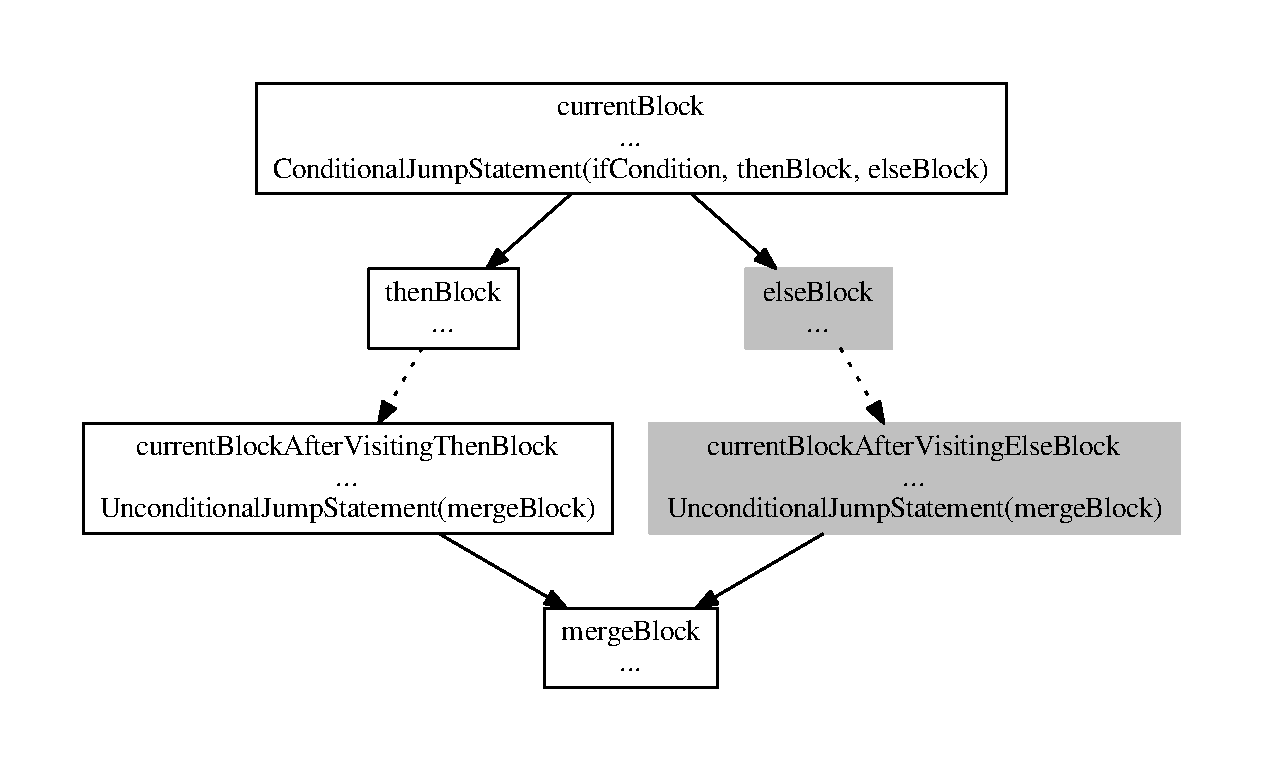
\includegraphics[width=\textwidth]{src/graph/graph.pdf}
    \caption{If statement CFG\label{img:if-statement}}
\end{figure}